\lab{Algorithm}{Invertible Affine Transformations}{Invertible Affine Transformations}
\label{lab:ChangeBasis}

\objective{Understand how to apply various linear affine transformations to 
a set of vectors.}


\section*{Basis}

Recall that \emph{basis} for a vector space is a linearly independent set of vectors
that spans the entire space. Given a basis, it is possible to express
every vector in the space as a unique linear combination of the basis vectors
(indeed, this property can be taken as the definition for a basis).
Bases themselves are not necessarily unique, however, and it can often be
very useful to change the basis representation of vectors, both in theory and
practice. Changing basis is an example of an important class of mappings
known as \emph{linear transformations}.

In finite dimensional vector spaces like $\mathbb{R}^n$, any linear
transformation can be implemented as a single left matrix multiplication.
In other words, a mapping $T : \mathbb{R}^n \to \mathbb{R}^n$ is linear if and
only if there exists an $n \times n$ matrix $A$ such that $T\left(X\right) = AX$
for all vectors $X \in \mathbb{R}^n$.
If $P$ is an $n \times m$ matrix of points $m$ points in $\mathbb{R}^n$ and $A$
is the $n \times n$ matrix representation of a linear transformation, then $AP$
is the matrix of transformed points.
Different sorts of linear transformations can be represented by different types
of matrices.

In this lab we will take vectors in $\mathbb{R}^2$ and apply various linear and
affine transformations.
For all these exercises we will use the points:
\begin{lstlisting}
 pts = np.array([-1.5,-1.,-.5,0.,.5,1.,1.5,.75,-.75],
                [0.,-1.,-2.,-2.,-2.,-1.,0.,2.,2.])
\end{lstlisting}
In this case we have represented each point as a column of the array \li{pts}.
It is common to represent points as rows as well.
In that case, the transformations described below can still be performed by
transposing the arrays in the appropriate places.

\section*{Dilation}
Dilation, or scaling, is a type of linear transformation in which, from a
geometrical perspective, points are stretched or compressed.
The matrix representation $A$ of a dilation is a diagonal matrix. The values
on the main diagonal indicate the amount of stretching in their respective
directions.
\begin{figure}
\centering
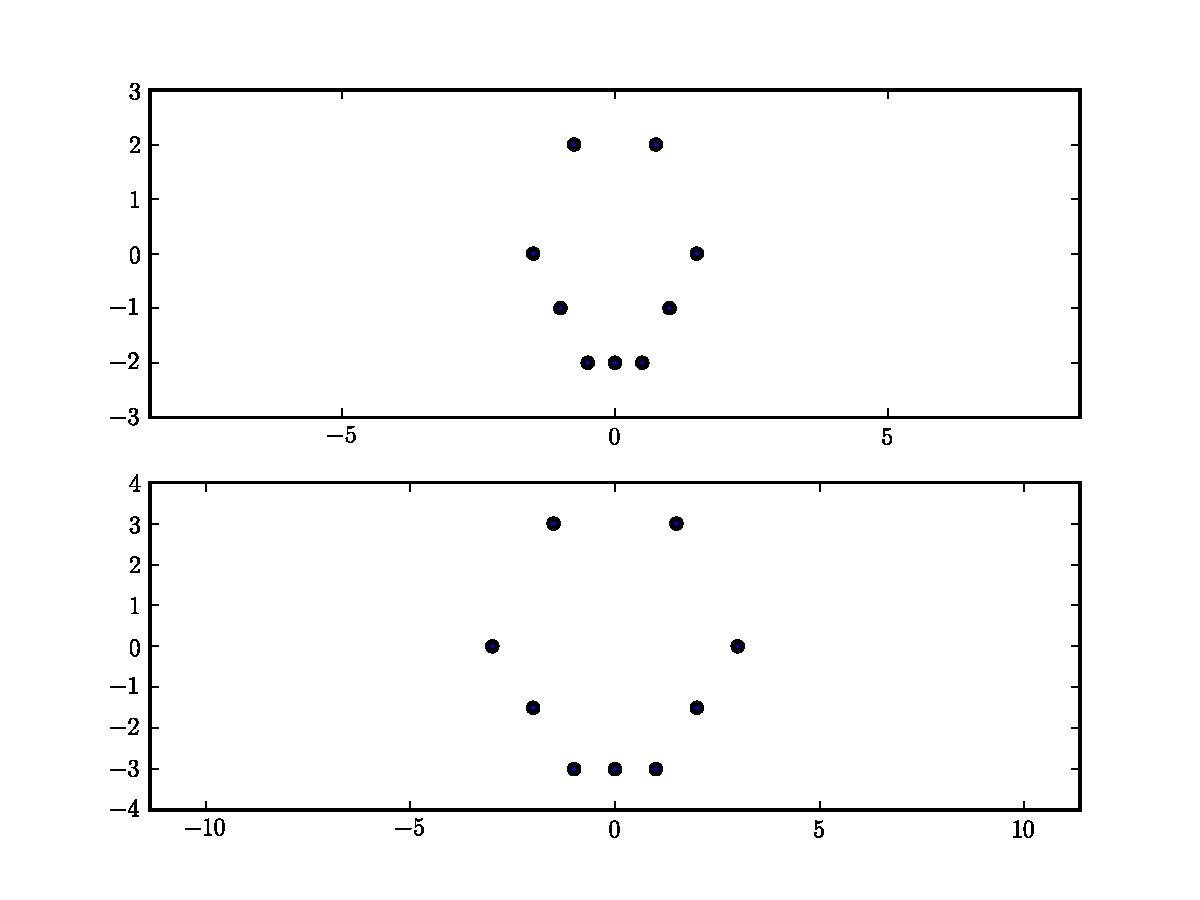
\includegraphics[width=\textwidth]{stretch.pdf}
\caption{
An example of a dilation. The top image is the original image and the bottom is
the modified image.
The figure was stretched by a factor of $2$ in the $x$ direction and $1.5$ in
the $y$ direction.}
\end{figure}

\begin{problem}
Write a function that accepts an array of points and an array giving the
stretching factors in each direction, and returns the dilated points.
Plot the original points and their image under the transformation.
This can be done with the following code:
\begin{lstlisting}
# assume that the arrays 'old' and 'new'
# have x values along the first row and
# y values along the second row
from matplotlib import pyplot as plt
plt.subplot(2, 1, 1)
plt.scatter(old[0], old[1])
plt.axis('equal')
plt.subplot(2, 1, 2)
plt.scatter(new[0], new[1])
plt.show()
\end{lstlisting}
\end{problem}

\section*{Rotation}
Rotating points around the origin is another type of linear transformation.
To perform a rotation of $\theta$ radians counterclockwise, let
\[
A = \begin{pmatrix}
\cos(\theta) & -\sin(\theta) \\
\sin(\theta) & \cos(\theta)
\end{pmatrix}
\]

\begin{figure}
\centering
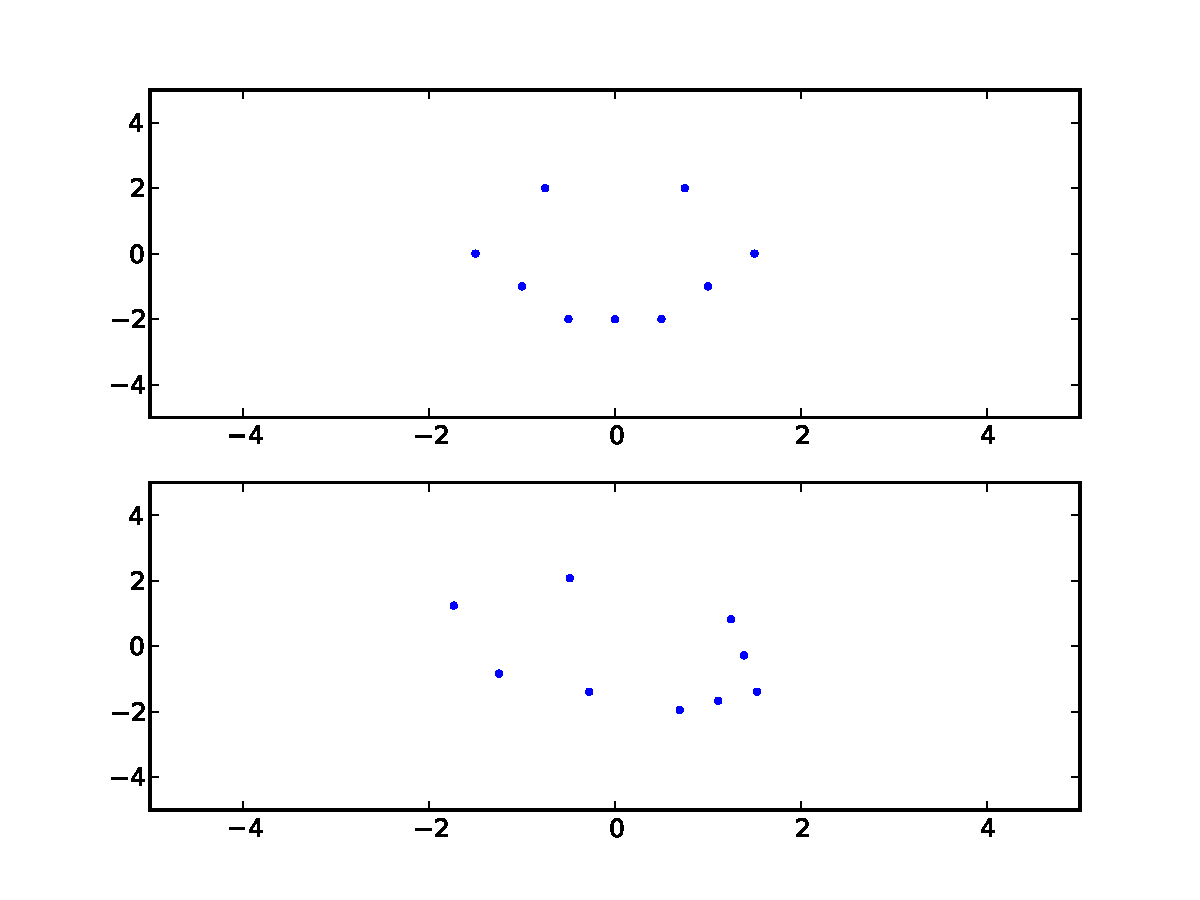
\includegraphics[width=\textwidth]{rotate.pdf}
\caption{An example of a rotation.
The top image is the original and the bottom is the rotated image.
The rotation angle is $\frac{3\pi}{16}$.}
\label{basis:rotate}
\end{figure}

\begin{problem}
Write a function that accepts an array of points and the angle of rotation (in
radians). Have it return the rotated points.
Plot the original points and their image under the transformation.
\end{problem}

\section*{Shear}

\begin{figure}
\centering
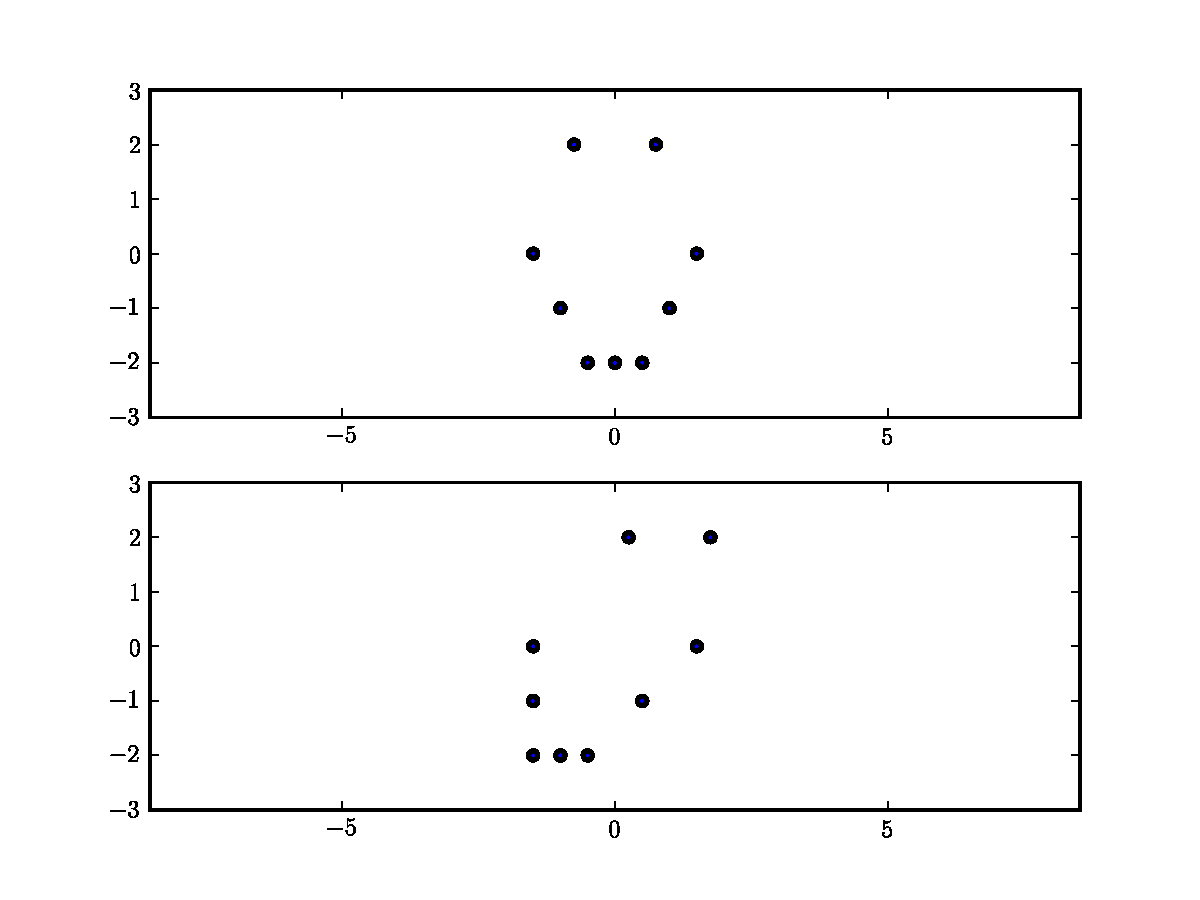
\includegraphics[width=\textwidth]{shear.pdf}
\caption{An example of a shear.
The top image is the original and the bottom is the sheared image.}
\label{basis:shear}
\end{figure}

A shear is a linear transformation that displaces a vector in a fixed direction.
In $\mathbb{R}^2$, a shear can either be horizontal or vertical, and has one of
the two following forms, respectively:
\[
A = \begin{pmatrix}
1 & c \\
0 & 1
\end{pmatrix}
\]
\[
A = \begin{pmatrix}
1 & 0 \\
c & 1
\end{pmatrix},
\]
where $c$ indicates the amount of displacement. As you can see in Figure \ref{basis:shear},
a sheared figure looks like the original figure viewed from an angle. Note that
these shearing matrices are instances of a type III elementary matrix. Horizontal
shears leave the y-coordinates fixed, while vertical shears leave the x-coordinate
fixed. In physics, shears are known as Galilean Transformations, and are used
to switch between reference frames that differ only by constant relative motion.

\begin{problem}
Write a function that accepts an array of points and an integer argument
that indicates the direction of shearing (0 for horizontal, 1 for vertical).
Have it return the sheared points.
Plot the original points and their image under the transformation.
\end{problem}

\section*{Reflection}
\begin{figure}
\centering
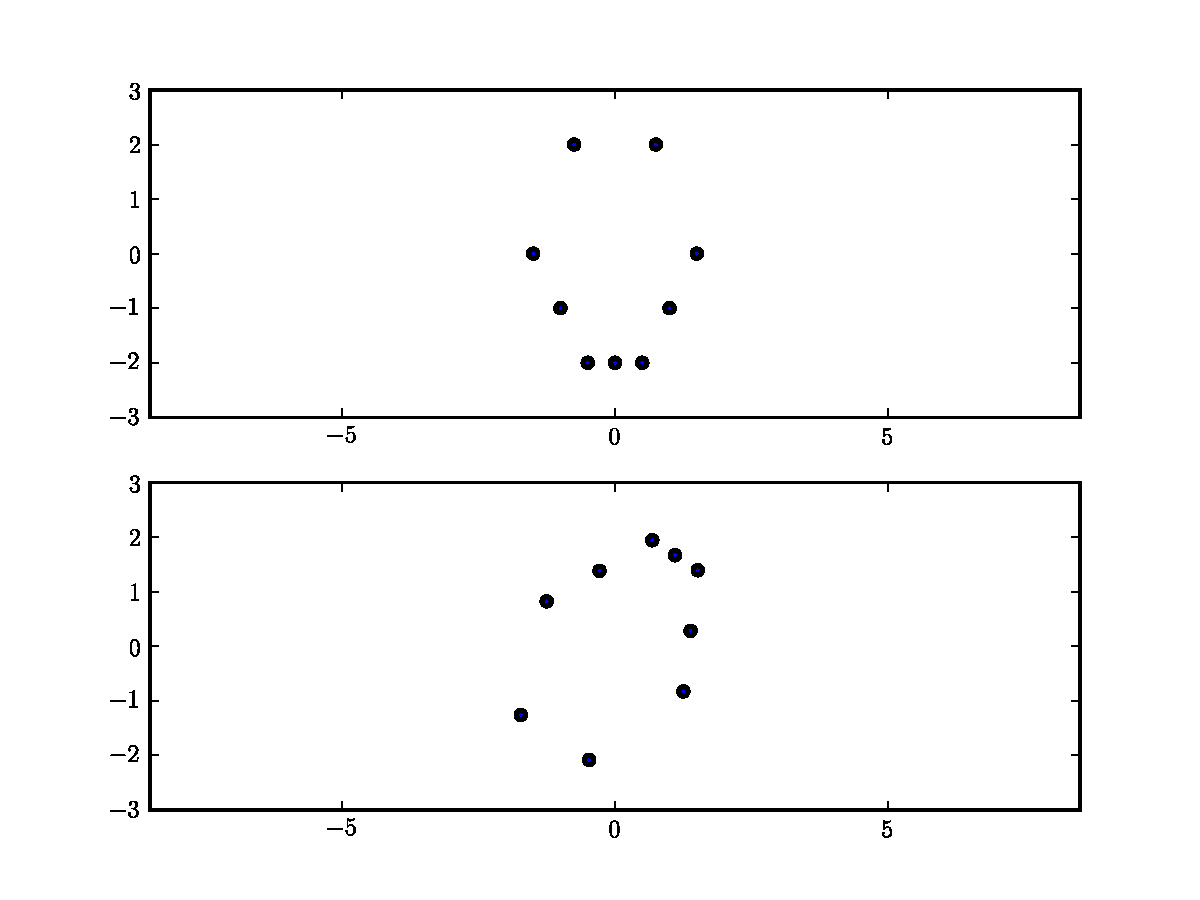
\includegraphics[width=\textwidth]{reflection.pdf}
\caption{An example of a reflection.
The top image is the original and the bottom is the image after
being reflected about the line $y = -3x$.}
\label{basis:reflection}
\end{figure}
Reflection about a line (or in higher-dimensional spaces, a hyperplane) can also be
accomplished by a linear transformation. Such a transformation is called a
\emph{Householder Transformation}, and the general form of the matrix representation in
$\mathbb{R}^2$ is
\[
A = \frac{1}{l_1^2 + l_2^2}
\begin{pmatrix}
l_1^2 - l_2^2 & 2l_1l_2 \\
2l_1l_2 & l_2^2 - l_1^2
\end{pmatrix},
\]
where $(l_1, l_2)$ is a vector in the direction of the axis of reflection. In the simple
case where the axis of reflection is the line $y=x$, the matrix is just a Type I elementary
matrix. See Figure \ref{basis:reflection} for an example.

\begin{problem}
Write a function that accepts an array of points and an array giving the axis of
reflection (in the notation above, this argument is $(l_1, l_2)$.
Have it return the reflected points.
Plot the original points and their image under the transformation.
\end{problem}

\section*{Translation}

\begin{figure}
\centering
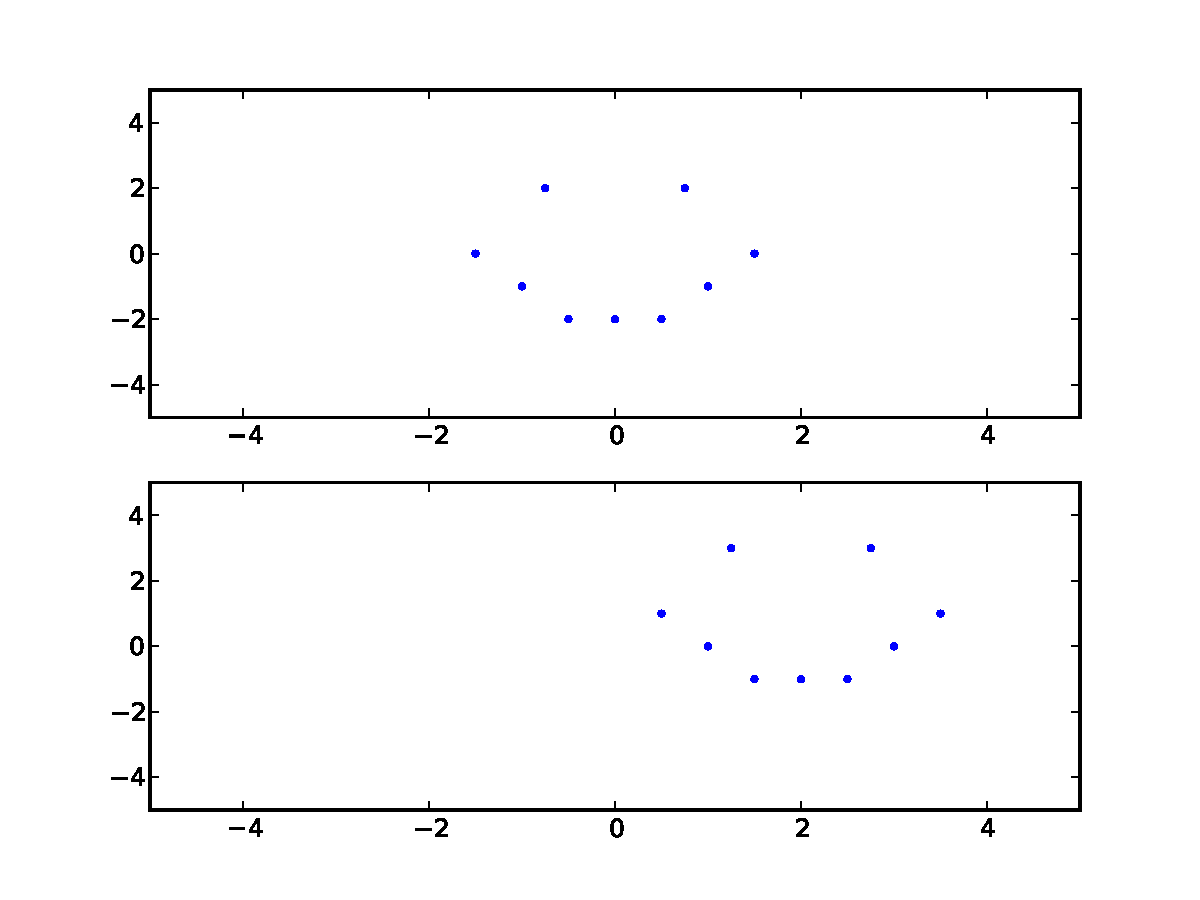
\includegraphics[width=\textwidth]{shift.pdf}
\caption{
An example of a translation.
The top image is the original and the bottom is the modified image.}
\label{basis:translation}
\end{figure}

Translations are not linear transformations, but they can be performed easily with array operations.
Together with linear transformations, they make up the broader class of transformations called
``affine transformations."
These are transformations of the form $T: \mathbb{R}^n \to \mathbb{R}^n$, $T(X) = AX + b$ where $A$ is
an $n\times n$ matrix and $b \in \mathbb{R}^n$.
Affine transformations include all compositions of scalings, rotations, and translations.


Let $b$ be a vector that represents the desired translation.
In order to shift a set of points, you add to the row how much you would like it to shift
in that direction. Thus, to shift the set of points up by 2, simply add \li{b = np.array([[0], [2]])}.
This particular shape for $b$ allows for proper array broadcasting.
See Figure \ref{basis:translation} for an example.

\begin{problem}
Write a function that takes an array of points and an array indicating how much to shift
them in each direction. The function should return the translated points.
Plot the original points and their image under the transformation.
\end{problem}

\section*{Compositions of Transformations}
\begin{figure}
\centering
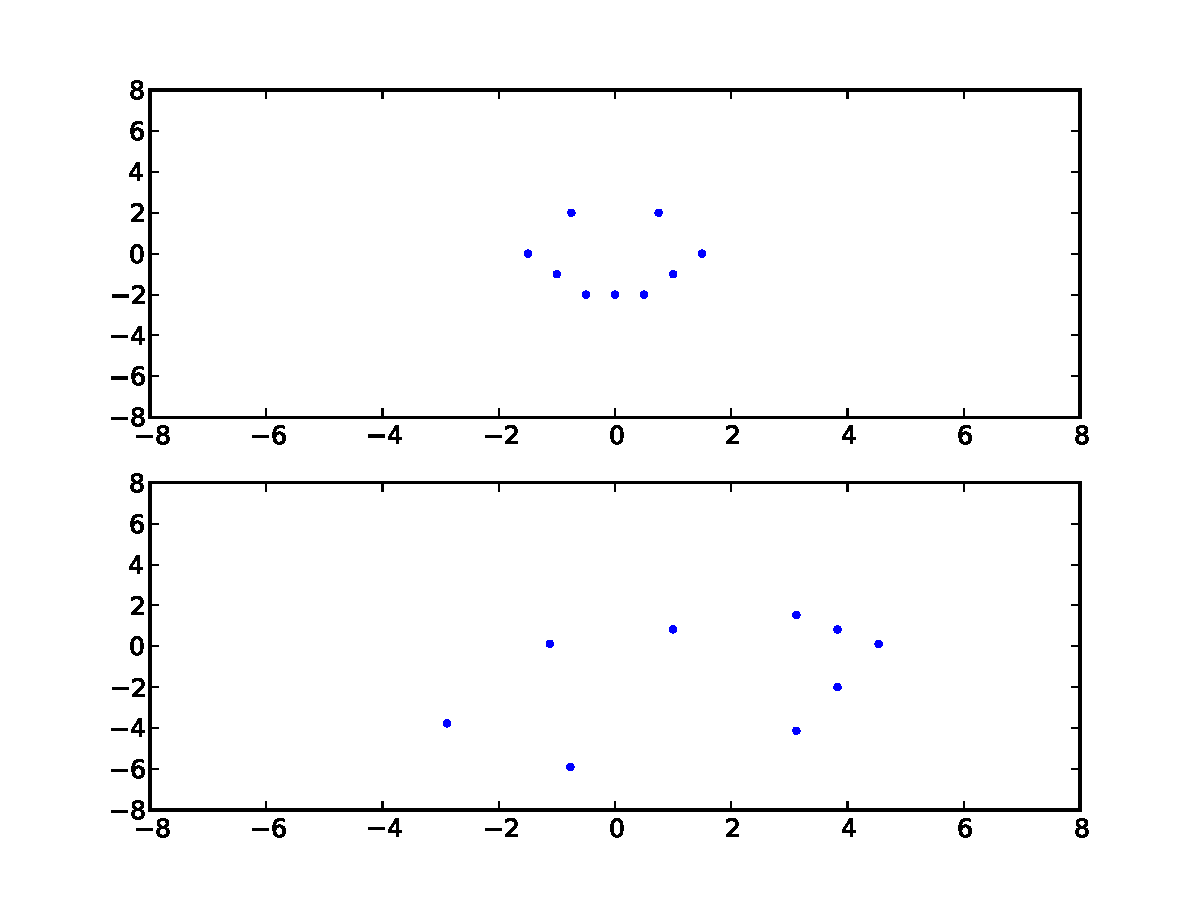
\includegraphics[width=\textwidth]{combo.pdf}
\caption{
A composition of linear transformations: scaling, rotation, and translation.}
\label{basis:combo}
\end{figure}
These transformations can be combined into single affine transformations through function composition.
For example, if you want to apply a scaling and then a rotation, you can represent the
scaling as a matrix $S$ and the rotation as a matrix $R$. The combined transformation is then $RS$.
The image of $X$ under both transformations will be $RSX$.
An example like this is shown in Figure \ref{basis:combo}.

\begin{problem}
We can use affine transforms to track the trajectory of a particle $p_1$ that rotates about
another particle $p_2$ at a constant angular speed $\omega$ (a positive value means
counterclockwise rotation), while $p_2$ moves in a particular
direction at a constant speed $v$. Suppose that $p_2$ has a starting position at the origin and
moves in the direction of the vector $(1, 1)$, and suppose that $p_1$ has a starting position
at the point $(0,1)$. Write a function that takes three parameters giving the time, angular
velocity, and directional speed, respectively, and returns the position of $p_1$ at that time.

Visualize a trajectory by plotting the position of the particle at each time (in seconds) in the array
\li{times = numpy.arange(0,10,.1)} for an angular velocity $\pi$ radians per second and a
directional speed of 3 meters per second (assume the plot is on a meters scale).
\end{problem}

